\section{The VM Placement Problem}
\label{sec:vmpp}

A VMPP can be summarized in three-steps (see Figure
\ref{fig:scheduling_steps}): monitoring the resources usages,
computing a new schedule each time is it needed and applying the
resulting reconfiguration plan (\ie performing VM migration and
suspend/resume operations to realize to the new placement solution).
% that are mandatory to solve resource violations while optimizing resource usages).

\begin{figure}[ht]
\vspace*{-.2cm}
\begin{center}
        \subcapcentertrue
        \subfigure[Scheduling steps]{
        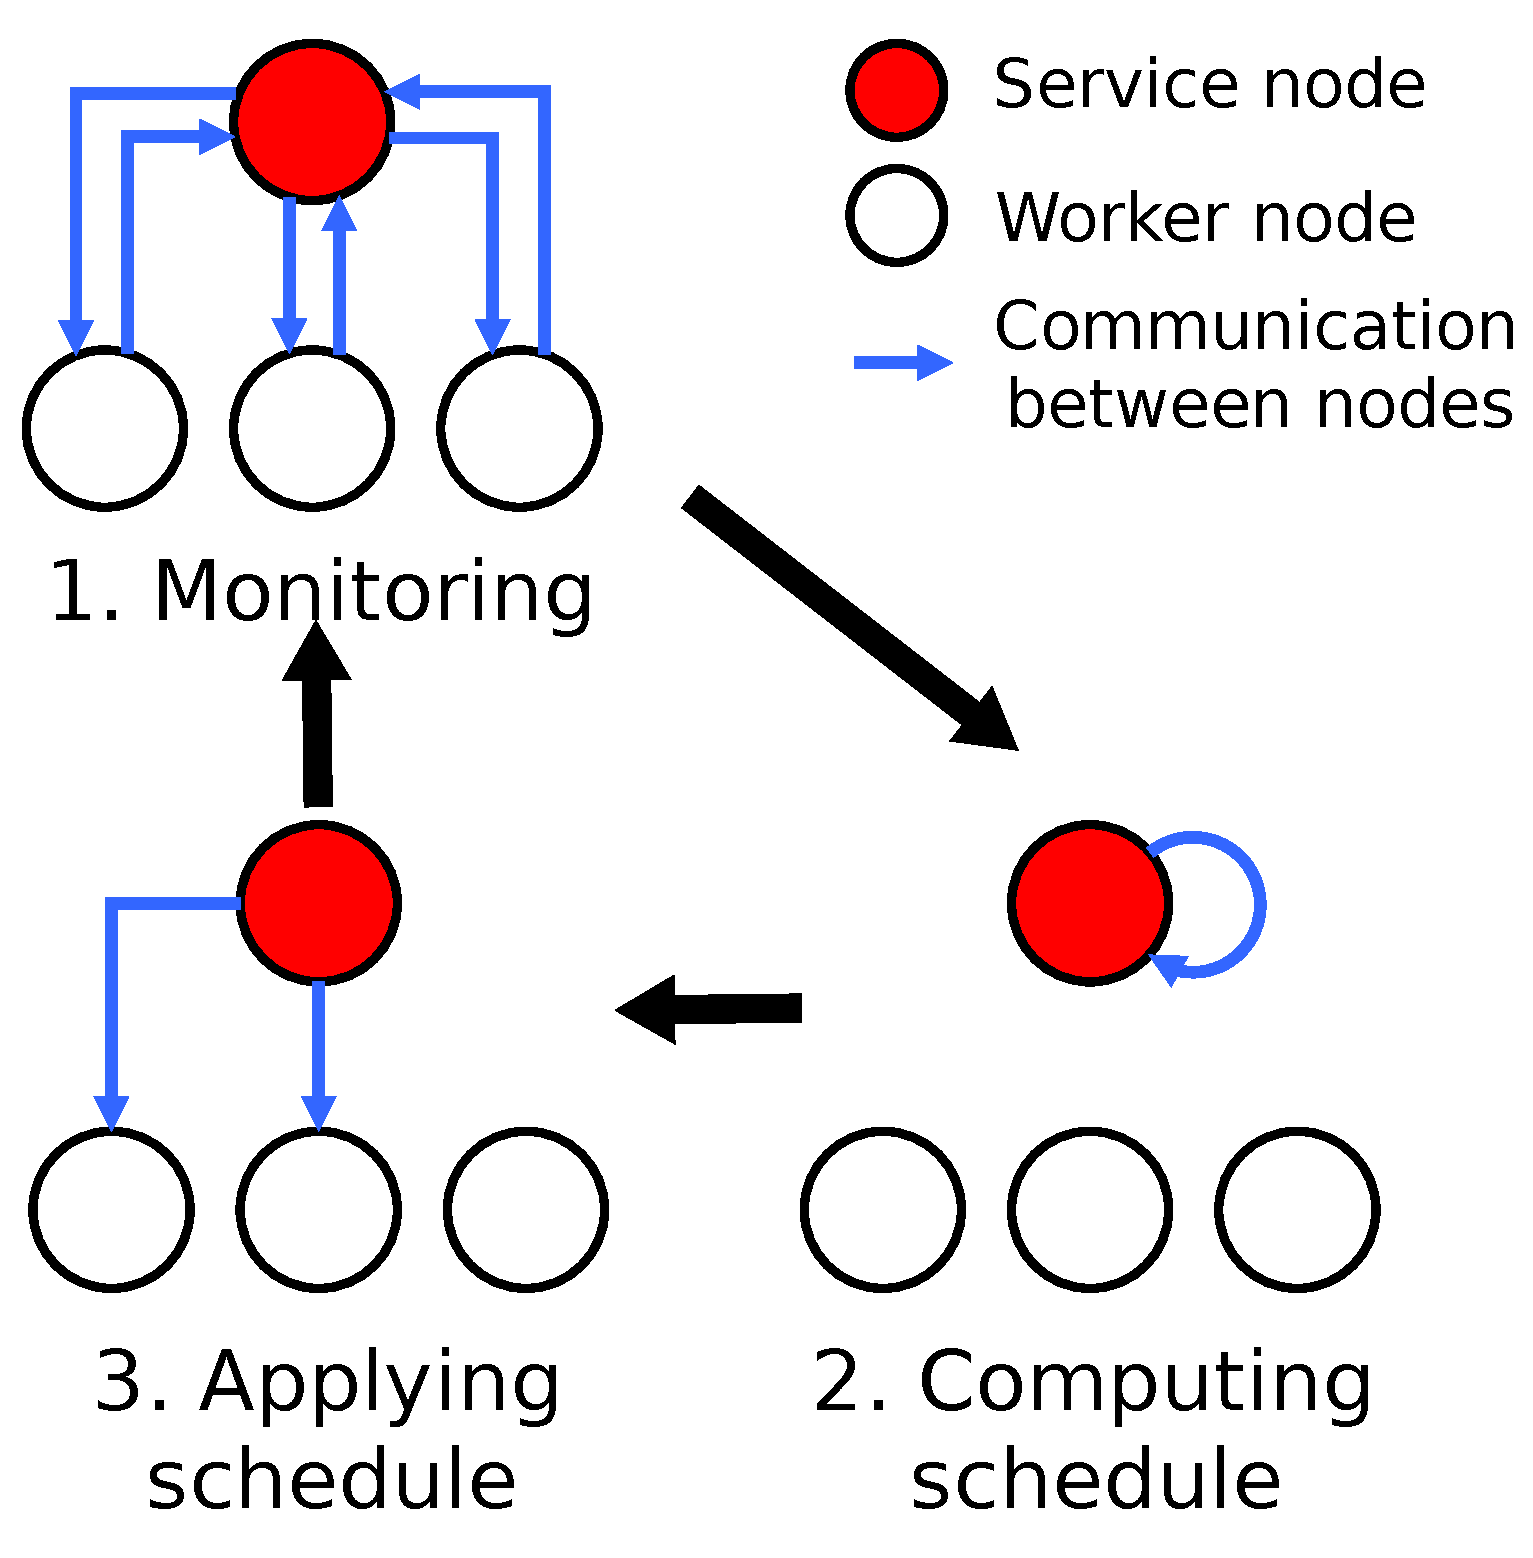
\includegraphics[width=.45\linewidth]{figures/scheduling_steps.pdf}
        \label{fig:scheduling_steps}}
        \subfigure[Workload fluctuations during scheduling]{
        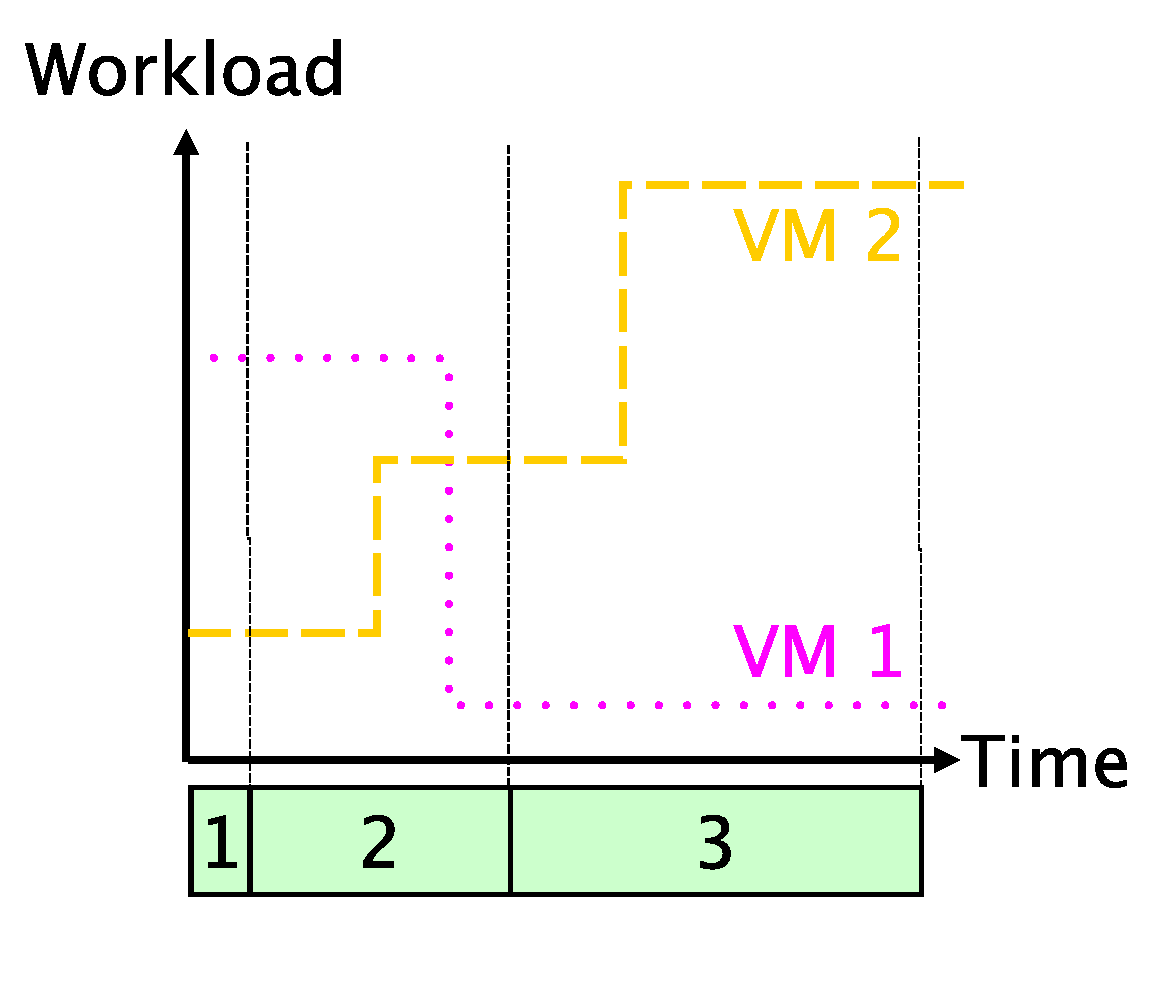
\includegraphics[width=.45\linewidth]{figures/workload_fluctuations2.pdf}
        \label{fig:workload_fluctuations}}
\vspace*{-.2cm}
\caption{VM scheduling Phases}
\end{center}
\label{fig:scheduling}
\vspace*{-.2cm}
\end{figure}
%

VMPP solutions stand and fall with their scalability, reliability and
reactivity of properties, because they have to maintain a placement
that satisfies the requirements of all VMs while optimizing the usage
of CC resources. For instance, a naive implementation of a
master/worker approach as described in
Figure~\ref{fig:scheduling_steps} would prevent workload fluctuations
to be taken into account during the computation and the application of
a schedule, potentially leading to artificial violations (\ie resource
violations that are caused by the VMPP mechanism). In other words, the
longer each phase,
% the longer the reconfiguration process,
the higher the risk that the schedule may be outdated when it is
computed or eventually applied, cf.\ the different loads during the
three phases in Figure \ref{fig:workload_fluctuations}. Similarly,
servers and network crashes can impede the detection and resolution of
resource violations if the master node crashes or if a group of VMs is
temporarily isolated from the master node.

VMPP solutions can only be reasonably evaluated if their behavior in
the presence of such adverse events can be analyzed. Providing a
framework that facilitates such studies and increases their
reproducibility is the main objective of \vmps.


